\documentclass[12pt]{article}
\usepackage[utf8]{inputenc}
\usepackage{float}
\usepackage{amsmath}
\usepackage{enumerate}
\usepackage{tikz}
\usepackage{tikz-qtree}
\usetikzlibrary{automata,positioning}
\usepackage{tabularx}

\usepackage[hmargin=3cm,vmargin=6.0cm]{geometry}
%\topmargin=0cm
\topmargin=-2cm
\addtolength{\textheight}{6.5cm}
\addtolength{\textwidth}{2.0cm}
%\setlength{\leftmargin}{-5cm}
\setlength{\oddsidemargin}{0.0cm}
\setlength{\evensidemargin}{0.0cm}

%misc libraries goes here
\usepackage{tikz}
\usetikzlibrary{automata,positioning}

\begin{document}

\section*{Student Information} 
%Write your full name and id number between the colon and newline
%Put one empty space character after colon and before newline
Full Name : Zeynep Özalp \\
Id Number : 2237691
% Write your answers below the section tags
\section*{Answer 1}

\subsection*{a.}
\begin{enumerate}[(i)]
\item
$G=\{V,\Sigma,R,S\}$\\
$V=\{a,b,S,S_1,S_2\}$\\
$\Sigma=\{a,b\}$\\
$R=\{S->aSa|bS_1, \\
S_1->aS_1a|b \}$
\item 
E generates the strings of even length except the empty sting, O generates the strings of odd length. The length of string produced by S is $even+even+3=odd$ or $odd+odd+3=odd$.\\
$G=\{V,\Sigma,R,S\}$\\
$V=\{a,b,S,E,O\}$\\
$\Sigma=\{a,b\}$\\
$R=\{S->aEaEa|bEbEb|aOaOa|bObOb|aaa|bbb, \\
E->aEa|aEb|bEa|bEb|aa|bb, \\
O->aE|Ea|bE|Eb|a|b \}$
\item
$S_1$ creates the string $a^ib^jc^k$ where $i\neq j$ and $S_2$ creates the string $a^ib^jc^k$ where $j\neq k$. For $S_1$, $T_1$ creates the string $a^ib^j$ where $i\neq j$. $T_2$ creates the string $a^ib^j$ where $i=j$. $A_1$ is $a^+$, $B_1$ is $b^+$ and $C_1$ is $c^*$. For $S_2$, $T_3$ creates the string $b^jc^k$ where $j\neq k$. $T_4$ creates the string $b^jc^k$ where $k=j$. $A_2$ is $a^*$, $B_2$ is $b^+$ and $C_2$ is $c^+$. \\
$G=\{V,\Sigma,R,S\}$\\
$V=\{a,b,S,S_1,S_2,T_1,T_2,T_3,T_4,A_1,A_2,B_1,B_2,C_1,C_2\}$\\
$\Sigma=\{a,b\}$\\
$R=\{
S -> S_1 | S_2, \\
S_1 -> T_1C_1, \\
T_1 -> A_1T_2 | T_2B_1, \\
T_2 -> aT_2b | e, \\
A_1 -> aA_1, \\
B_1 -> bB_1, \\
C_1 -> cC_1 | e, \\
S_2 -> A_2T_3, \\
T_3 -> B_2T_4 | T_4C_2, \\
T_4 -> bT_4c | e, \\
B_2 -> bB_2, \\
C_2 -> cC_2, \\
A_2 -> aA_2 | e
\}$
\item 
$S_1$ generates all strings, $S_2$ generates a $w_ic$, $S_3$ generates the sequence of $w_ic$'s. $S_4$ generates $w_jc\{sequence of w_ic's\}cw_j^R$.\\
$G=\{V,\Sigma,R,S\}$\\
$V=\{a,b,S,S_1,S_2,S_3,S_4\}$\\
$\Sigma=\{a,b\}$\\
$R=\{S->S_3S_4, \\
S_1->aS_1|bS_1|e, \\
S_2->aS_1c|bS_1c, \\
S_3->S_2S_3|S_2, \\
S_4->aS_4a|bS_4b|cS_3c \}$
\end{enumerate}

\subsection*{b.}
\subsubsection*{PART 1}
$L(G)\subseteq L$, every string generated by G is in L. \\
Use mathematical induction. \\\\
1. Basis step: Derivation in 2 steps.
$$S\Rightarrow aB\Rightarrow ab \in L$$
$$S\Rightarrow bA\Rightarrow ba \in L$$\\
2. Inductive Hypothesis: Assume that for every derivation $S\Rightarrow^* w$ with $n\geq2$ steps, $w\in L$\\\\
3. Inductive Step: Let $S\Rightarrow^*w$ be a derivation with $n+2$ steps, $n\in N$. Since $n+2> 2$, the derivation starts with either $abS,baS,aABB$ or $bBAA$.\\\\
i)$S\Rightarrow aB\Rightarrow abS \Rightarrow^* abw_1$. By ind. hyp., $w_1\in L$,$w_1$ has equal number of a's and b's, so does $abw_1$ and $abw_1 \in L$.\\
ii)$S\Rightarrow bA\Rightarrow baS \Rightarrow^* baw_2$. By ind. hyp., $w_2\in L$,$w_2$ has equal number of a's and b's, so does $baw_2$ and $baw_2 \in L$.\\
iii)$S\Rightarrow aB\Rightarrow abS \Rightarrow abaB\Rightarrow abaABB$. So, the string $aABB$ can be generated by $S$ in two steps and in $L$. \\
iv)$S\Rightarrow bA\Rightarrow baS \Rightarrow babA\Rightarrow babBAA$. So, the string $bBAA$ can be generated by $S$ in two steps and in $L$. \\
Therefore, every string generated by G is in L.
\subsubsection*{PART 2}
$L\subseteq L(G)$, every string in L can be generated by G. \\
$L=\{ab,ba,...\}$
Use mathematical induction. \\\\
1. Basis step: For $|w|=2$, $S \Rightarrow aB \Rightarrow ab$ and $S \Rightarrow bA \Rightarrow ba$. So, $ab \in L(G)$ and $ba \in L(G)$.\\\\
2. Inductive Hypothesis: Assume that all strings $|w| \leq k-1$ in L can be generated by G.\\\\
3. Inductive Step: Suppose $x=a_1a_2a_3...a_k \in L$ with $k>2$, $a_i\in \Sigma$. Now assume that $a_1a_2=ab$. Define $N_a(x)$ as the number of a's in x and 
$$d_i=N_a(x)-N_b(x), 0\leq i \leq k$$
$$t=min(i>0, d_i=0)$$

Since we choose $a_1a_2 = ab$, $ d_1 = 1, d_2=0$. Also, $d_k = 0$ since $x \in L$. Thus, there exists a smallest i such that $d_i=-1$ and $d_{i+1}=0$. This value is represented as t. Since t was chosen to be the smallest possible and $d_1>0$, we must have $d_t<0$. Since $d_t<0$ and $d_{t+1}=0$, we must have $a_ta_{t+1} = ba$. Therefore, we have
$$x=aba_3...a_{t-1}baa_{t+2}...a_k$$
Let $y=a_3...a_{t-1}$ and $z=a_{t+2}...a_k$. Clearly, because $x\in L$, y and z have equal number of a's and b's, $y \in L$ and $z \in L$. By inductive hypothesis, since $|y|<k$ and $|z|<k$, $y,z \in L(G)$. This means $S\Rightarrow ^* y$ and $S\Rightarrow ^* z$.
$$S\Rightarrow aB \Rightarrow abS \Rightarrow ^* abyS \Rightarrow  abybA \Rightarrow abybaS \Rightarrow ^* abybaz = x$$ 
Therefore, $x\in L(G)$ and for all $x\in L \rightarrow x\in L(G)$. This completes the proof that $L(G)$ is the set of all non-empty strings in $\Sigma^*$ that have equal number of a's and b's.

\section*{Answer 2}

\subsection*{a.}
% Sample empty trees for your convenience, edit/use as you wish
$$s=aab$$
$S\Rightarrow aaB \Rightarrow aab$\\
$S\Rightarrow Ab \Rightarrow Aab \Rightarrow aab$\\

\begin{minipage}[c]{\textwidth}
\hfill
\Tree [.S [.a ] [.a ] [.B b ]]
\hspace{0.2\linewidth}
\Tree [.S [.A [.A a ] [.a ] ] [.b ] ]
\hspace{0.3\linewidth}
\end{minipage}

\subsection*{b.}
$L(G)=\{ab,aab,aaab,...\}$\\
G' is an equivalent unambiguous CFG of G.\\
$G'=\{V', \Sigma, R', S\}$, $V'=\{a,b,S,A\}$,\\
$R=\{S\rightarrow Ab, A\rightarrow a|aA\}$

\subsection*{c.}
% Sample empty tree for your convenience, edit/use as you wish
\Tree [.S [.A [.A a ] [.a ] ] [.b ] ]
\section*{Answer 3}

\subsection*{a.}
$L=\{w\in \{a,b\}^*|w=(aa)^i(bbb)^i, i\geq 0\}$
\subsection*{b.}
$M=\{K,\Sigma,\Gamma, \Delta, q_0, q_7\}$\\
$K=\{q_0,q_1,q_2,q_3,q_4,q_5,q_6,q_7\}$, $\Sigma=\{a,b\}, \Gamma=\{Z_0,X,Y\}$\\
$T=\{Z_0,X\}$\\

% Sample empty diagram for your convenience, edit/use as you wish.
\tikzset{every loop/.style={min distance=10mm,looseness=10}}
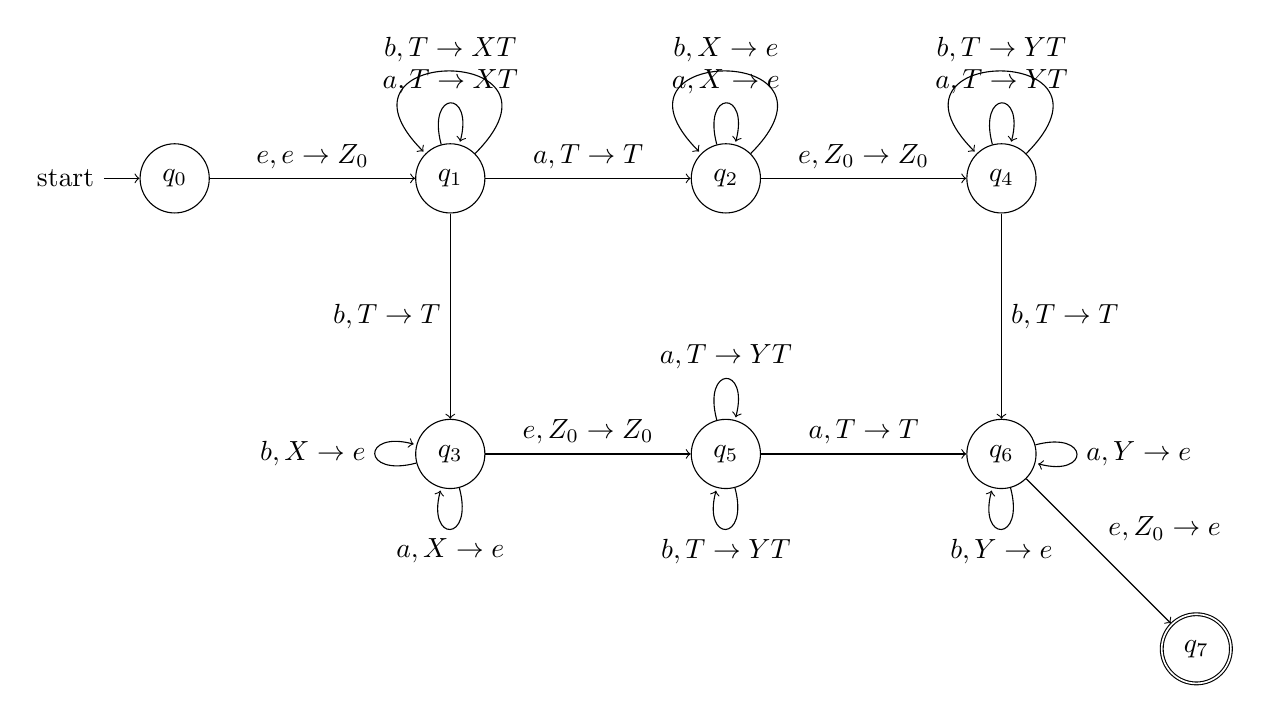
\begin{tikzpicture}[node distance=3.5cm,on grid,auto] 
\node[state,initial] (q_0) {$q_0$}; 
\node[state] (q_1) [right of=q_0] {$q_1$}; 
\node[state] (q_2) [right of=q_1] {$q_2$}; 
\node[state] (q_3) [below of=q_1] {$q_3$}; 
\node[state] (q_4) [right of=q_2] {$q_4$}; 
\node[state] (q_5) [below of=q_2] {$q_5$}; 
\node[state] (q_6) [below of=q_4] {$q_6$}; 
\node[state,accepting] (q_7) [below right of=q_6] {$q_7$}; 
\path[->]
  (q_0) edge node {$e,e\rightarrow Z_0$} (q_1)
  (q_1) edge [loop=90 above, swap] node {$b,T\rightarrow XT$} () edge [loop above] node {$a,T\rightarrow XT$} () edge node {$a,T\rightarrow T$} (q_2) edge [swap] node {$b,T\rightarrow T$} (q_3)
  (q_2) edge [loop=90 above, swap] node {$b,X\rightarrow e$} () edge [loop above] node {$a,X\rightarrow e$} () edge node {$e,Z_0\rightarrow Z_0$} (q_4)
  (q_3) edge [loop left] node {$b,X\rightarrow e$} () edge [loop below] node {$a,X\rightarrow e$} () edge node {$e,Z_0\rightarrow Z_0$} (q_5)
  (q_4) edge [loop=90 above, swap] node {$b,T\rightarrow YT$} () edge [loop above] node {$a,T\rightarrow YT$} () edge node {$b,T\rightarrow T$} (q_6)
  (q_5) edge [loop below] node {$b,T\rightarrow YT$} () edge [loop above] node {$a,T\rightarrow YT$} () edge node {$a,T\rightarrow T$} (q_6)
  (q_6) edge [loop below] node {$b,Y\rightarrow e$} () edge [loop right] node {$a,Y\rightarrow e$} () edge node {$e,Z_0 \rightarrow e$} (q_7)
  ;
\end{tikzpicture}
\\\\\\
\subsection*{c.}
\begin{enumerate}[(i)]
\item 
$L(M)=\{a^ib^jc^k\in \{a,b,c\}^*|i,j,k\geq 0, i=j$ or $j>k$ or $j<k\}$\\
$M=(K, \{a,b,c\}, \Gamma, \Delta, q_0, \{q_3,q_7\})$\\
$K=\{q_0,q_1,q_2,q_3,q_4,q_5,q_6,q_7,q_8,q_9,q_{10}\}$, $\Gamma=\{Z_0,a,b\}$\\

\begin{tabular}{c} %for alignment purposes
% Sample empty diagram for your convenience, edit/use as you wish.
\tikzset{every loop/.style={min distance=10mm,looseness=10}}
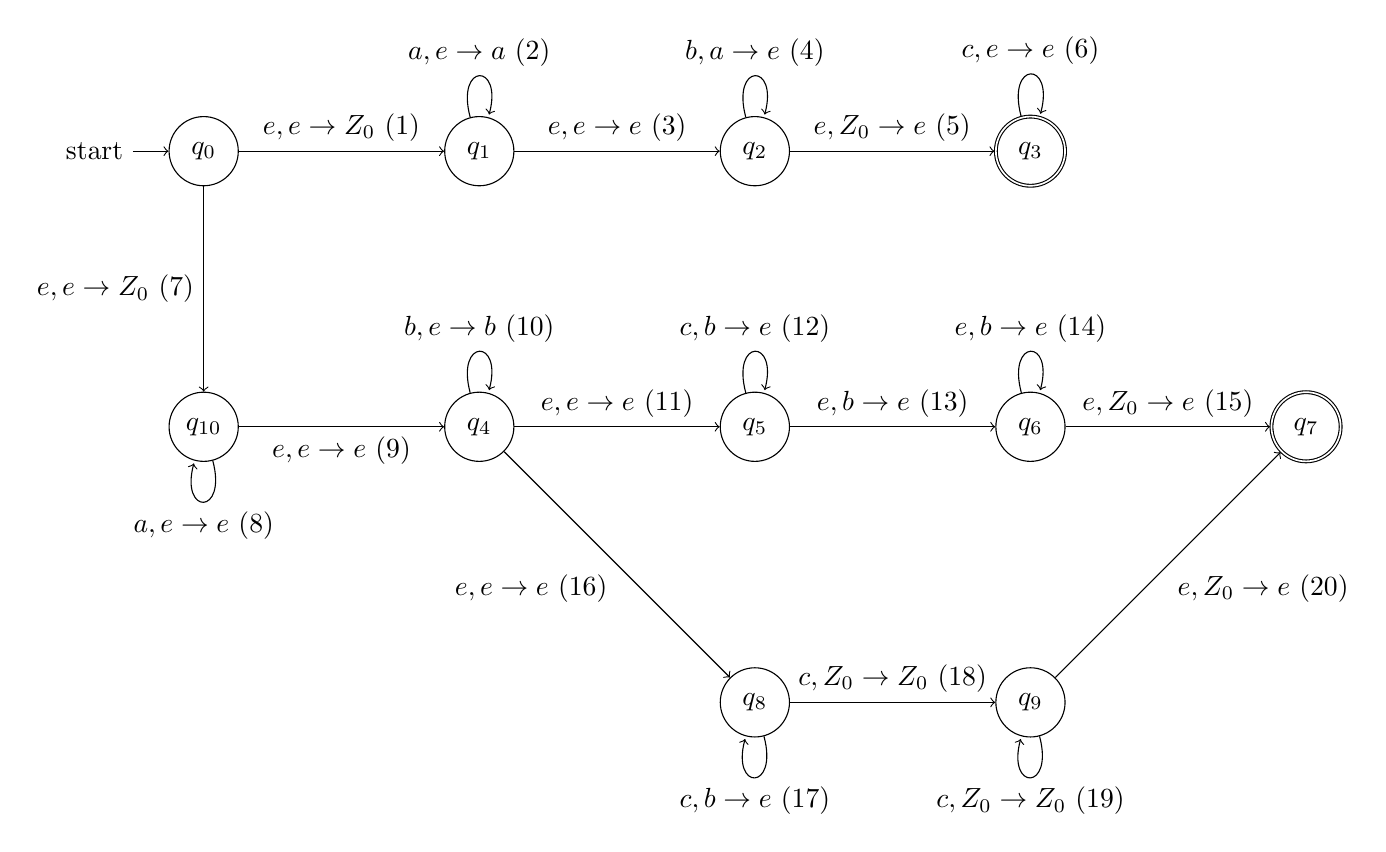
\begin{tikzpicture}[node distance=3.5cm,on grid,auto] 
\node[state,initial] (q_0) {$q_0$};
\node[state] (q_1) [right of=q_0] {$q_1$}; 
\node[state] (q_2) [right of=q_1] {$q_2$};
\node[state,accepting] (q_3) [right of=q_2] {$q_3$};
\node[state] (q_4) [below of=q_1] {$q_4$};
\node[state] (q_5) [right of=q_4] {$q_5$};
\node[state] (q_6) [right of=q_5] {$q_6$};
\node[state,accepting] (q_7) [right of=q_6] {$q_7$};
\node[state] (q_8) [below of=q_5] {$q_8$};
\node[state] (q_9) [below of=q_6] {$q_9$};
\node[state] (q_{10}) [below of=q_0] {$q_{10}$};
\path[->]
  (q_0) edge node {$e,e\rightarrow Z_0$ (1)} (q_1) edge [swap] node {$e,e\rightarrow Z_0$ (7)} (q_{10})
  (q_1) edge [loop above] node {$a,e\rightarrow a$ (2)} () edge node {$e,e\rightarrow e$ (3)} (q_2)
  (q_2) edge [loop above] node {$b,a\rightarrow e$ (4)} () edge node {$e,Z_0\rightarrow e$ (5)} (q_3)
  (q_3) edge [loop above] node {$c,e\rightarrow e$ (6)} ()
  (q_4) edge [loop above] node {$b,e\rightarrow b$ (10)} () edge node {$e,e\rightarrow e$ (11)} (q_5) edge [swap] node {$e,e \rightarrow e$ (16)} (q_8)
  (q_5) edge [loop above] node {$c,b\rightarrow e$ (12)} () edge node {$e,b\rightarrow e$ (13)} (q_6)
  (q_6) edge [loop above] node {$e,b\rightarrow e$ (14)} () edge node {$e,Z_0\rightarrow e$ (15)} (q_7)
  (q_8) edge [loop below] node {$c,b\rightarrow e$ (17)} () edge node {$c,Z_0\rightarrow Z_0$ (18)} (q_9)
  (q_9) edge [loop below] node {$c,Z_0\rightarrow Z_0$ (19)} () edge [swap] node {$e,Z_0\rightarrow e$ (20)} (q_7)
  (q_{10}) edge [loop below] node {$a,e\rightarrow e$ (8)} () edge [swap] node {$e,e\rightarrow e$ (9)} (q_4)
  ;
\end{tikzpicture}
\end{tabular}

\item 
% Sample empty table for your convenience, edit/use as you wish.
\begin{tabular}{|llrl|}
\hline
State & Input & Stack & Transition\\
$q_0$ & aabcc & e     &  - \\
$q_{10}$ & aabcc & $Z_0$ & (7) \\
$q_{10}$ & abcc  & $Z_0$     & (8) \\
$q_{10}$ & bcc   & $Z_0$     & (8) \\
$q_4$ & bcc   & $Z_0$     & (9) \\
$q_4$ & cc   & $b,Z_0$     & (10) \\
$q_8$ & cc   & $b,Z_0$     & (16) \\
$q_8$ & c   & $Z_0$     & (17) \\
$q_9$ & e  & $Z_0$     & (18) \\
$q_7$ & e   & e     & (20) \\
$q_7$ & e   & e     & Accepts. \\

\hline
\end{tabular}
% Sample empty table for your convenience, edit/use as you wish.
% You are expected to trace all the possible computations
\begin{tabular}{|llrl|}
\hline
State & Input & Stack & Transition \\
$q_0$ & bac & e & - \\
$q_1$ & bac & $Z_0$ & (1) \\
$q_2$ & bac & $Z_0$ & (3) \\
$q_3$ & bac & $Z_0$ & (5) \\
$q_3$ & bac & $Z_0$ & Rejects. \\
\hline
$q_0$ & bac & e & - \\
$q_{10}$ & bac & $Z_0$ & (7) \\
$q_4$ & bac & $Z_0$ & (9) \\
$q_4$ & ac & $b,Z_0$ & (10) \\
$q_5$ & ac & $b,Z_0$ & (11) \\
$q_5$ & ac & $b,Z_0$ & Rejects. \\
\hline
$q_0$ & bac & e & - \\
$q_{10}$ & bac & $Z_0$ & (7) \\
$q_4$ & bac & $Z_0$ & (9) \\
$q_4$ & ac & $b,Z_0$ & (10) \\
$q_8$ & ac & $b,Z_0$ & (11) \\
$q_8$ & ac & $b,Z_0$ & Rejects. \\
\hline
\end{tabular}
\end{enumerate}


\section*{Answer 4}

\subsection*{a.}
Construct a PDA $M=( \{p,q\} ,\Sigma ,V,\Delta ,p,\{q\})$ such that $L(M)=L(G)$. By Lemma 3.4.1, \\
$\Delta = \\
((p,e,e),(q,E)),\\
((q,e,E),(q,E+T)),\\
((q,e,E),(q,T)),\\
((q,e,T),(q,T\times F)),\\
((q,e,T),(q,F)),\\
((q,e,F),(q,(E))),\\
((q,e,F),(q,a)),\\
((q,a,a),(q,e)),\\
((q,+,+),(q,e)),\\
((q,\times,\times),(q,e)),\\
((q,(,(),(q,e)),\\
((q,),)),(q,e))\\$

\subsection*{b.}
First add $\Delta '$ the transitions ((s',e,e),(s,Z)) and ((f,e,Z),(f',e)) for each $f\in F$. Now, $\Delta '$ consists of these transitions described above and all the transitions in $\Delta$. Next, we replace all the transitions in $\Delta '$ that violates the condition $|\beta|+|\gamma|\leq 1$. \\

Consider any transition $((q,a,\beta),(p,e))$ where $\beta=B_1B_2...B_n$ with $n>1$. It is replaced by new transitions that pop sequentially the symbols $B_1...B_n$. So, we add $\delta '$ these transitions:
$$((q,e,B_1),(q_1,e))$$
$$((q_1,e,B_2),(q_2,e))$$
$$\vdots$$
$$((q_{n-2},e,B_{n-1}),(q_{n-1},e))$$
$$((q_{n-1},e,B_n),(p,e))$$
We repeat these replacements for all transitions $((q,a,\beta),(p,e))$ where $|\beta|>1$ in $\delta '$.\\

Similarly, we replace transitions $((q,a,e),(p,\gamma))$ where $\gamma=G_1G_2...G_m$ and $m>1$ by the new transitions:
$$((q,e,e),(q_1,G_1))$$
$$((q_1,e,e),(q_2,G_2))$$
$$\vdots$$
$$((q_{n-2},e,e),(q_{n-1},G_{n-1}))$$
$$((q_{n-1},e,e),(p,G_n))$$
We repeat these replacements for all transitions $((q,a,e),(p,\gamma))$ where $|\gamma|>1$ in $\delta '$.\\

Now, consider any transition $((q,a,\beta),(p,\gamma))$ where $\beta=B_1B_2...B_n$ with $n>1$ and $\gamma=G_1G_2...G_m$ with $m>1$. We replace these transitions by the new transitions:
$$((q,e,B_1),(q_1,e))$$
$$((q_1,e,B_2),(q_2,e))$$
$$\vdots$$
$$((q_{n-2},e,B_{n-1}),(q_{n-1},e))$$
$$((q_{n-1},e,B_n),(p,e))$$
$$((q_n,e,e),(q_{n+1},G_1))$$
$$((q_{n+1},e,e),(q_{n+2},G_2))$$
$$\vdots$$
$$((q_{n+m-2},e,e),(q_{n+m-1},G_{m-1}))$$
$$((q_{n+m-1},e,e),(p,G_m))$$
It is clear that the resulting pushdown automata is equivalent to the original one.

\section*{Answer 5}

\subsection*{a.}
\begin{enumerate}[(i)]
\item 
Let $L_1=\{a^m b^m \in \{a,b\}^* |m\in N\}$ and $L_2=\{b^n a^n \in \{a,b\}^* |n\in N\}$. Grammer for $L_1$ is $G_1=\{\{a,b,S\},\{a,b\}, \{S\rightarrow aSb|e\},S\}$ and grammer for $L_2$ is $G_1=\{\{a,b,S\},\{a,b\}, \{S\rightarrow bSa|e\},S\}$. So, $L_1$ and $L_2$ are context-free languages. By Theorem 3.5.1, their concatenation $L_1L_2$ are also context-free.

\item 
$L=\{ba,babaa,babaabaaa,...\}$\\
Let $L'$ be the complement of $L$ and use an algorithm to find the complement of $L$. We can generate strings that is not in $L$ by changing one $a$ or $b$ from the beginning and in order. For $n=1$, we have the string $ba$ in $L$. Change a $b$ to an $a$ or change an $a$ to a $b$ in $ba$, we get $aa$ or $bb$ respectively, which are not in $L$. Concatenating $\Sigma^*$ to these two strings we have the languages $aa\Sigma^*$ and $bb\Sigma^*$. These two languages differ from $L$ by the first $a$ or the first $b$ symbols. However, we may have other strings that differs from $L$ by changing the $n^th$ $a$ to a $b$ and $n^th$ $b$ to an $a$, which are in case, the ones who do not fit the condition of $L$. Thus, one can generate $L'$ by taking the infinite union of such languages.
$$L'=a\Sigma^*\cup baa\Sigma^*\cup babaaa\Sigma^*\cup ...\cup bb\Sigma^*\cup babb\Sigma^*\cup babab\Sigma^*\cup babaabb\Sigma^*\cup ...$$
Since all regular languages are context-free and context-free languages are closed under union by Theorem 3.5.1, $L'$ is context-free.
\end{enumerate}

\subsection*{b.}
\begin{enumerate}[(i)]
\item 
Assume L is context-free. Then there exists a pumping length $k$ such that for all $w\in L$ and $|w|>k$ there exists a split $w=uvxyz$, $|vy|>0$, $|vxy|\leq k$ and $yv^nxy^nz\in L$ for all $n\geq 0$. Choose $w=a^{k^2}b^k$. There are three possible splits:\\\\
\textbf{1)} $vxy=a^j$, $j>0$. $uv^2xy^2z=a^{k^2+2j}b^k$. $k^2+2j$ is not less than or equal $k^2$ since $j>0$. \\
\textbf{2)} $vxy=b^j$, $j>0$. $uv^2xy^2z=a^{k^2}b^{k+2j}$. $k^2$ is not less than or equal $(k+2j)^2$ since $j>0$. \\
\textbf{3)} $vxy=a^ib^j$, $0<i+j\leq k$. There are 2 cases:\\
3.1) $v$ and $y$ consist of one symbol, $v=a^l$ and $y=b^m$. If we pump n times, we get $a^{k^2+nl}b^{k+nm}$. $k^2+nl\leq (k+nm)^2$ should hold for all $n,m,l\in N$. Clearly it does not.\\
3.2) One of $v$ or $y$ consist of two symbols, say v, $v=a^ib^j$ and $y=b^m$. When we pump, the order of the new string does not match the order of the languages in $L$ that is first only a's then only b's.\\
For all of these 3 cases, $w\notin L$. Thus, L is not context-free.

\item 
Assume L is context-free. Then there exists a pumping length $k$ such that for all $www\in L$ and $|www|>k$ there exists a split $www=uvxyz$, $|vy|>0$, $|vxy|<k$ and $yv^nxy^nz\in L$ for all $n\geq 0$. Choose $www=a^kb^ka^kb^ka^kb^k$. There are three possible splits:\\\\
\textbf{1.} $vxy=a^i$. For n=0:\\
1.1: $yv^nxy^nz=a^{k-i}b^ka^kb^ka^kb^k$ is not in L since to get w we need to split this string in 3 pieces with equal lengths. However, when we do this, the first one ends with an a but the last one ends with a b. So, there no such string in L.\\
1.2: $yv^nxy^nz=a^kb^ka^{k-i}b^ka^kb^k$ is not in L since to get w we need to split this string in 3 pieces with equal lengths. However, when we do this, the first one begins with an a but the middle one begins with a b. So, there no such string in L.\\
1.3: $yv^nxy^nz=a^kb^ka^kb^ka^{k-i}b^k$ is not in L since to get w we need to split this string in 3 pieces with equal lengths. However, when we do this, the first one begins with an a but the last one begins with a b. So, there no such string in L.\\ 
The same discussion and reasons are valid for case 2 and 3.\\
\textbf{2.} $vxy=a^ib^j$. For n=0:\\
2.1: $yv^nxy^nz=a^{k-i}b^{k-j}a^kb^ka^kb^k$\\
2.2: $yv^nxy^nz=a^kb^ka^{k-i}b^{k-j}a^kb^k$\\
2.3: $yv^nxy^nz=a^kb^ka^kb^ka^{k-i}b^{k-j}$\\
\textbf{3.} $vxy=b^ja^i$. For n=0:\\
3.1: $yv^nxy^nz=a^kb^{k-j}a^{k-i}b^ka^kb^k$\\
3.2: $yv^nxy^nz=a^kb^ka^kb^{k-j}a^{k-i}b^k$\\
Therefore, L is not context-free.

\end{enumerate}


\section*{Answer 6}
% You do not need to explain the following
\begin{enumerate}[(i)]
\item (T/F)? F
\item (T/F)? T
\item (T/F)? T
\item (T/F)? F
\end{enumerate}

% Please do not submit your answers to the ungraded questions.
% Hope you have fun :) 
\end{document}

​

